\chapter{Problem and Approaches to Solution}

% Problem: Wie sauber die Wahrscheinlichkeiten darstellen? Ein Produkt wird dann gekauft, wenn ein Customer eines bestimmten Segments kommt (lambda_l) und der Customer dann das Produkt auch kauft (p_lj)

\section{The problem}

Here, we want to lay out the classical revenue management problem an the \enquote{brute force} approach to solve. 

Consider a firm that produces products $j = 1, \dots, n$ with revenues $\boldsymbol{r} = (r_1, \dots, r_n)^T$. Resources $h = 1, \dots, m$ are used for production. In order to produce one unit of product $j$, resources $\boldsymbol{a}_j = (a_{1j}, \dots, a_{mj})^T$ are necessary, with $a_{hj}=1$ if resource $h$ is needed for production of product $j$ and $a_{hj} = 0$ otherwise. Initially, the capacity is described by $\boldsymbol{c}^0 = (c_1^0, \dots, c_m^0)^T$. 

The booking horizon is modelled by sufficiently small time periods $t = 0, \dots, T-1$, such that in each time period at most one customer arrives. This customer also purchases at most one product. If product $j$ is purchased at time $t$, the capacity reduces to $\boldsymbol{c}^{t+1} = \boldsymbol{c}^t - \boldsymbol{a}_j$. Time moves forward, such that the last selling might occur at time $T-1$.

The firm wants to increase the value of the products sold and has flexibility in the sets offered. Thus, the decision variables at each time point $t$ are given by $\boldsymbol{x}^t = (x^t_1, \dots, x^t_n)^T$ with $x^t_j = 1$ if product $j$ is offered at time $t$ and $x^t_j = 0$ otherwise. Thus, at each time point $t$ and each capacity $\boldsymbol{c}$, the offer set $\boldsymbol{x}$ has to be determined. Note that in machine learning terms, this mapping is defined as a policy $\boldsymbol{\psi} = (\psi^1, \dots, \psi^T)^T$.

One popular method of describing the probabilities of purchases is to have each customer belonging to one customer segment $l = 1, \dots L$, each of which following a multinomial logit model (MNL\nomenclature{MNL}{multinomial logit model}). A customer of segment $l$ arrives with probability $\lambda_i$. His preference weights are given by $\boldsymbol{u}_l = (u_{l1}, \dots, u_{ln})^T$ and no purchase preference of $u_{l0}$. Note: $u_{lj} > 0$ if consumer of segment $l$ might purchase product $j$ (the higher, the more interested) and $u_{lj} = 0$ if customer is not interested in product. The probability of purchasing product $j$ when set $\boldsymbol{x}$ is offered is given by $p_{lj}(\boldsymbol{x}) = \frac{u_{lj}x_j}{u_{l0} + \sum_{p\in[n]} u_{lp}x_p}$ and the no-purchase probability is given by $p_{l0}(\boldsymbol{x}) = 1 - \sum_{j\in[n]}p_{lj}$. Together with the uncertainty of which customer segment arrives (if any), we end up at a purchase probability for product $j$ given $\boldsymbol{x}$ of $p_j(\boldsymbol{x}) = \sum_{l \in [L]} \lambda_l p_{lj}(\boldsymbol{x})$ and a no purchase probability of $p_0(\boldsymbol{x}) = 1-\sum_{j\in[n]}p_j(\boldsymbol{x}) $. Thus, $p_j(\boldsymbol{x})$ can be interpreted as the deterministic quantity of product $j$ being sold, if set $\boldsymbol{x}$ is offered.

\subsection{Dynamic Programming}

The first solution approach might be to maximize the expected value of all revenues to gain given period $t$ and capacity $\boldsymbol{c}$, denoted by the value function $V^t(\boldsymbol{c})$. This can then be computed recursively as

\begin{align}
	V^t(\boldsymbol{c}) &= \max_{x^t \in \{0,1\}^n}\left\{ \sum_{j \in [n]} p_j(x_t) \left( r_j + V^{t+1}(\boldsymbol{c} - \boldsymbol{a}_j) \right) + p_0 V^{t+1}(\boldsymbol{c}) \right\} \label{eq-Bellman}\\
	&= \max_{x^t \in \{0,1\}^n}\left\{ \sum_{j \in [n]} p_j(x_t) \left( r_j - \Delta_j V^{t+1}(\boldsymbol{c}) \right) \right\} + V^{t+1}(\boldsymbol{c})\quad \forall t, \boldsymbol{c} \geq 0
\end{align}

with $\Delta_j V^{t+1}(\boldsymbol{c}) := V^{t+1}(\boldsymbol{c}) - V^{t+1}(\boldsymbol{c} - \boldsymbol{a}_j)$ and boundary conditions $V^{T+1}(\boldsymbol{c}) = 0$ if $\boldsymbol{c} \geq \boldsymbol{0}$ and $V^t(\boldsymbol{c}) = - \infty$ if $\boldsymbol{c} \ngeq \boldsymbol{0}$.

The optimal offerset $^*\boldsymbol{x}^t$ is then given by

\begin{align}
	^*\boldsymbol{x}^t = \argmax_{x^t \in \{0,1\}^n}\left\{ \sum_{j \in [n]} p_j(x_t) \left( r_j - \Delta_j V^{t+1}(\boldsymbol{c}) \right) \right\} + V^{t+1}(\boldsymbol{c})\quad \forall t, \boldsymbol{c} \geq 0\label{eq-DP-optOffer}
\end{align}

The resulting value function can be plotted in a three dimensional plot as done in \Cref{fig-valueFunc}.

\begin{figure}
\caption{\label{fig-valueFunc} Value function of single leg flight example with $t \in [20]$ on x-axis, $c \in [12]$ on y-axis.}
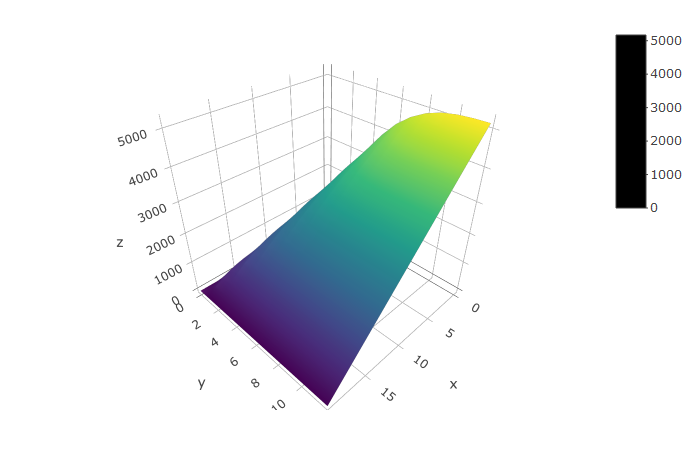
\includegraphics[width=\linewidth]{C:/Users/Stefan/LRZ Sync+Share/Masterarbeit-Klein/Code/Results/smallTest2-False-DP-190619-1333/value_function.png}
\end{figure}

\subsection{Dynamic Programming - Theory}

As this whole thesis is based on the ideas of Dynamic Programming, we want to give a short overview of the underlying mathematical theory and directly combine it to our setting.

Dynamic Programming (DP\nomenclature{DP}{dynamic programming}) refers to a broad collection of algorithms used to compute optimal policies given a perfect model of the environment as a Markov Decision Process (MDP\nomenclature{MDP}{markov decision process}), as stated in \cite{Sutton.2018}. A MDP is characterized by a state set $\mathcal{S}$ (the varying capacities $\mathbf{c}$ together with the current point in time $t$), an action set $\mathcal{A}$ (the offer sets $\mathbf{x}$) and reward sets $\mathcal{R}$ (the revenue $r$ if a product is sold). A MDP evolves over time, but for the evolution from time $t$ to $t+1$ only the current state $s_t$ is relevant and the history of previous states $s_h, h<t$ can be ignored. The dynamic is given by a set of probabilities $p(s', r | s, a)$ (capacities reduce according to which random product the random customer has bought according to his preferences). 

The goal of DP is to determine the optimal policy, i.e. which action to choose at each given state. Key to the solution is the usage of value functions as seen above. These fulfil the Bellman optimality equations as stated in \Cref{eq-Bellman}. 

%TODO elaborate on curse of dimensionality
In our setting, uniqueness of the optimal value function is ensured, as the MDP is guaranteed to terminate under any policy because time is moving forward no matter which action we choose, compare \cite{Sutton.2018}. Thus, while the problem can be solved, due to large scale decision problems and the curse of dimensionality, we are lacking computing power to solve it exactly and have to come up with approximate solution methods.

One approximate solution method is the usage of Approximate Policy Iteration (API\nomenclature{API}{approximate policy iteration}), which consists of two steps. The policy evaluation step (inner loop \Cref{alg-API-Peval1} to \Cref{alg-API-Peval2}) evaluates a fixed policy over a set of sample paths $\omega_i, i = 1, \dots, I$. The policy improvement step (outer loop \Cref{alg-API-Piter1}, \Cref{alg-API-Piter2}, \Cref{alg-API-Piter3}) improves the policy over the iterations $k = 1, \dots, K$.



\subsection{Choice based linear programming}

based on Bront et al and van Ryzin.

Taking an eagle-eye perspective, the company has to decide which sets to offer in every single time period, but as the probabilities don't change over time, the specific time point when to offer one set is indistinguishable, we can aggregate over time. Let us introduce a few more notation to get a hand on this. Let $R(\mathbf{x})$ represent the expected revenue given offer set $\boldsymbol{x}$, i.e.

\begin{align}
	R(\boldsymbol{x}) = \sum_{j \in [n]} r_j p_j(x) \quad.
\end{align}

Furthermore, let $\boldsymbol{Q}(\boldsymbol{x}) = (Q_1(\boldsymbol{x}), \dots, Q_m(\boldsymbol{x}))^T$ denote the expected capacity being used, i.e. 

\begin{align}
	Q_h(\boldsymbol{x}) = \sum_{j \in [n]} a_{hj} p_j(\boldsymbol{x}) \quad.
\end{align}

We can denote the total time set $\boldsymbol{x}$ is offered by $t(\boldsymbol{x})$ and the set of all possible offersets as $N = \{0,1\}^n$ . Thus, we can formulate the choice-based linear program (CDLP) \nomenclature{CDLP}{choice-based linear program} as presented in van Ryzin and Liu. Here the optimization problem is solved by varying the decision variables $t(\boldsymbol{x})$.

\begin{align}
	V^{CDLP} = & \max \sum_{\boldsymbol{x}\in N} R(\boldsymbol{x}) t(\boldsymbol{x})\\
	\text{s.t. } & \sum_{\boldsymbol{x}\in N} Q_h(\boldsymbol{x}) t(\boldsymbol{x}) \leq c_h \quad, \forall h\\
	& \sum_{\boldsymbol{x}\in N} t(\boldsymbol{x}) \leq T~,\\
	& t(\boldsymbol{x}) \geq 0 \quad \forall \boldsymbol{x} \in N~.
\end{align}

Korrektheit getestet mit \texttt{C:\textbackslash{}Users\textbackslash{}Stefan\textbackslash{}LRZ Sync+Share\textbackslash{}Masterarbeit-Klein\textbackslash{}Code\textbackslash{}H\_CDLP\_single\_leg.py} - Example0 in settings
Ergebnisse in \texttt{ C:\textbackslash{}Users\textbackslash{}Stefan\textbackslash{}LRZ Sync+Share\textbackslash{}Masterarbeit-Klein\textbackslash{}Code\textbackslash{}Results\textbackslash{}example0-False-CDLPSingleLeg-190621-1808}

\section{Approximate Dynamic Programming}

\subsection{Approximate Policy Iteration}

ADP builds upon \Cref{eq-DP-optOffer} and approximates opportunity costs additively using bid prices $\pi_h(t, c_h)$, i.e. $\Delta_j V^{t+1}(\boldsymbol{c}) = \sum_{h \in [m]} a_{hj}\pi_{h}(t+1, c_h)$. Thus, the policy is given as the solution of

\begin{align}
^\pi \boldsymbol{x}^t = \argmax_{x^t \in \{0,1\}^n}\left\{ \sum_{j \in [n]} p_j(x_t) \left( r_j - \sum_{h \in [m]} a_{hj}\pi_{h}(t+1, c_h) \right) \right\} 
\end{align}

Thus, the policy is completely described by the bid prices $\pi_h(t, c_h) \forall t$.

Let us discuss the algorithm in depth. In the beginning (\Cref{alg-API1}), all parameters are set to zero which results in the greedy policy of offering the set resulting in the highest expected revenue (no consideration of costs). 

In each policy iteration $k$, the current policy is evaluated first. To do so, we use the current policy to evaluate $I$ random paths. \Cref{alg-API3} sets up the dataset for revenues to go $\hat{V}_t^i$ and remaining capacities $\mathbf{\hat{C}}_t^i$ for all times $t$ and sample paths $i$. 

For each sample path $i$, a storage unit for revenue $\hat{r}_t$ and capacities $\mathbf{\hat{c}}$ is created for all times $t$ (\Cref{alg-API5}). Furthermore, the capacity is set to the initial capacity in \Cref{alg-API6}.

For each point in time, the current capacity $\mathbf{\hat{c}}_t$ is stored in \Cref{alg-API8}, the current bid prices are calculated in \Cref{alg-API9} and used to determine the offerset $\mathbf{x}$ in \Cref{alg-API10}. More details on the determination of the offerset can be found in \Cref{sec-determineOfferset}. With, this, a sales event $j'$ is simulated and in case a product has been sold, the revenue is stored and capacity adjusted (note: the revenue thus belongs to $t$ and capacity will affect $t+1$) (\Cref{alg-API11} to \Cref{alg-API13}).

After simulating one sample path, the value function for this sample path $\hat{V}_t$ is updated for all times $t$ in \Cref{alg-API14}, and so are the capacities in line \Cref{alg-API15}.

With all the information from the $I$ sample paths the parameters $\left(\theta_t, \pi_t \right)$ are updated. Note that the old parameters are used as starting values and the current number of policy iterations $k$ is also passed to potentially take care of exponential smoothing. Thus, we have $(1+h)*T$ parameters ($theta_t$ and $\pi_t$) and $2TI$ data points. More details on the update of the parameters can be found in \Cref{sec-updateParameter}.

%TODO Visualisierung wann was stattfindet
Actions possible in $t = 0, \dots, T-1$.


\begin{algorithm}
	\caption{Approximate policy iteration}\label{alg-API}
	\begin{algorithmic}[1]
		\State Set $\theta_t = 0$ and $\mathbf{\pi}_t = \mathbf{0}$ $\forall t = 0, \dots, T-1$ \label{alg-API1}
		\For{\texttt{k = 1 to K}} \label{alg-API-Piter1}
		\State Set $\hat{V}_t^i = 0$ and $\mathbf{\hat{C}}_t^i = 0$ $\forall t = 0, \dots, T-1, \forall i = 1, \dots, I$\label{alg-API-Piter2}\label{alg-API3}
		\For{\texttt{i = 1 to I}}\label{alg-API-Peval1}
		\State Set $\hat{r}_t = 0$ and $\mathbf{\hat{c}}_t = 0$ $\forall t = 0, \dots, T-1$\label{alg-API5}
		\State Initialize $\mathbf{c} = \mathbf{c}^0$\label{alg-API6}
		\For{\texttt{t = 0 to T-1}}
		\State $\mathbf{\hat{c}}_t \coloneqq \mathbf{c}$\label{alg-API8}
		\State Compute $\mathbf{\pi}(t, \mathbf{c})$ \label{alg-API-calcPi}\label{alg-API9}
		\State Compute $\mathbf{x} = \text{determineOfferset}(\mathbf{\pi}(t, \mathbf{c}), \epsilon_t)$\label{alg-API10}
		\State Simulate a sales event $j' \in \{0, 1, \dots, n\}$\label{alg-API11}
		\If{$j' \in \{ 1, \dots, n\}$}
		\State $\hat{r}_t = r_{j'}$ and $\mathbf{c} = \mathbf{c} - \mathbf{a}_{j'}$\label{alg-API13}
		\EndIf
		\EndFor
		\State Compute $\hat{V}_t^i = \sum_{\tau = t}^{T}\hat{r}_t \quad \forall t = 0, \dots, T-1$\label{alg-API14}
		\State Assign $\mathbf{\hat{C}}_t^i = \mathbf{\hat{c}}_t \quad \forall t = 0, \dots, T-1$\label{alg-API15} \label{alg-API-Peval2}
		\EndFor
		\State $\left(\theta_t, \pi_t \right) = \text{updateParameters}\left(\hat{V}_t^i, \mathbf{\hat{C}}_t^i, \theta_t, \pi_t, k\right) \quad \forall t = 0, \dots, T-1, \forall i = 1, \dots, I$ \label{alg-API-updateParam}\label{alg-API-Piter3}
		\EndFor
		\Return {$\left(\theta_t, \pi_t \right)  \quad \forall t = 1, \dots, T$}
	\end{algorithmic}
\end{algorithm}


Overview of parameters:
\begin{enumerate}
	\item $\theta_t$	optimization parameter (offset)
	\item $\mathbf{\pi}_t$	optimization parameter (bid price for each resource)
	\item $\hat{V}_t = 0$	all sample revenues to go for each sample for each time
	\item $\mathbf{\hat{C}}_t = 0$	all sample available capacities for each sample for each resource for each time
	\item $r_t$	sample revenue generated at time $t$
	\item $\mathbf{c}$	available capacities for each resource at current time
	\item $\mathbf{c}^0$	starting capacities
	\item $\mathbf{x}$ offerset at current time
	\item $\epsilon_t$ epsilon used at current time
\end{enumerate}


\subsection{Greedy Heuristic to determine offerset}\label{sec-determineOfferset}

The following algorithm is based on the ideas of the greedy heuristic for the column generation subproblem outlined in \cite{Bront.2009}.

Our goal is to determine a reasonable set of products to offer in a fast manner. Thus, we use a heuristic and cut down the amount of products to consider as fast as possible.

%todo expand on exploration vs exploitation dilemma
The function $\text{determineOfferset}(\mathbf{\pi}, \epsilon)$ calculates the set to offer depending on the current bid prices $\mathbf{\pi}$ via the greedy algorithm layed out in \cite{Bront.2009}. To account for the exploration vs exploitation dilemma, an epsilon-greedy strategy is used. With a probability of $\epsilon/2$ either no product is offered at all or all products with positive contribution $r_j - \sum_{h \in [m]} a_{hj} \cdot \pi_h$ are offered. With a probability of $1-\epsilon$, the proper calculated set is offered.

\todoRed{Value Funktion gebuendelt dargestellt und ueberall mit $\lambda$. Vergleiche zu Bront et al. 4.2.2, wo in 3. ohne $\lambda$ und in 4.a mit $\lambda$.}

\begin{algorithm}
	\caption{Greedy Heuristic}\label{alg-GreedyHeuristic}
	\begin{algorithmic}[1] % [1] results in line numbers
		% Großes X verwendet, um Menge zu symbolisieren
		\State $\text{Value}(X) \coloneqq \sum_{l=1}^{L} \lambda_l \frac{\sum_{i \in X}(r_i - A_i^T\pi)u_{li}}{\sum_{i \in X}u_{li} + u_{l0}}$
		\State $S\coloneqq \emptyset,\quad S' \coloneqq \left\{j \in N : r_j - A_j^T\pi > 0\right\}$ \label{alg-L1}
		\State $j^* \coloneqq \arg\max_{j \in S'} \text{Value}(\{j\})$
		\Repeat
		\State $S \coloneqq S \cup \{j^*\},\quad S' \coloneqq S'\backslash\{j^*\}$
		\State $j^* \coloneqq \arg \max_{j \in S'} \text{Value}(S \cup \{j\})$
		\Until {$\text{Value}(S \cup \{j^*\}) \leq \text{Value}(S)$\\}
		\Return {$S$}
	\end{algorithmic}
\end{algorithm}

%todo Kommentiere den Algorithmus.
Let $S'$ be the set of products with positive reduced costs, i. \Cref{alg-L1}

\subsection{Update of parameters}\label{sec-updateParameter}
%todo Schreibweise der Funktion anpassen, da alle Parameter auf eimal übergeben werden, und nicht separat je Zeitschritt
The function $\left(\theta_t, \pi_t \right) = \text{updateParameters}\left(\hat{V}_t, \mathbf{\hat{C}}_t, \theta_t, \pi_t, k\right)$ really optimizes the following least squares optimization problem for all parameters ($t = 1, \dots, T$) at the same time.

\begin{align}
V_t(\theta_t, \mathbf{\pi}_t, \mathbf{c}_t) & \coloneqq \theta_t + \sum_{h=1}^{m}\sum_{s=1}^{S_h} \pi_{ths} f_{hs}(c_h) \\
f_{hs}(c_h) &\coloneqq 
\begin{cases}\label{def-f}
0 & \text{ if } c_h \leq b_h^{s-1}\\
c_h - b_h^{s-1} & \text{ if } b_h^{s-1} < c_h \leq b_h^s \\
b_h^s - b_h^{s-1} & \text{ if } b_h^s < c_h
\end{cases}
\end{align}

\Cref{def-f} describes the occupied amount of capacity of interval $\left(b_h^{s-1}, b_h^s\right]$.

The following optimization problem depends on the old parameters $\theta_t = \theta_t^k$ and $\mathbf{\pi}_t = \mathbf{\pi}_t^k$ to determine the optimal parameter $\theta_t^{update}$ and $\mathbf{\pi}_t^{update}$.

\begin{alignat}{2}
& \text{min} \sum_{i=1}^{I}\sum_{t=1}^{T} \left( \hat{V}_t^i - V_t(\theta_t, \mathbf{\pi}_t, \mathbf{c}_t^i) \right)^2 && \\
& s.t. && \\
& \theta_t \geq 0 && \forall t\\
& \max_{j=1, \dots, n} r_j \geq \pi_{ths} \geq 0 && \forall t, h, s\\
& \pi_{ths} \geq \pi_{th,s+1} && \forall t, h, s = 1, \dots, S_h-1\\
& \theta_t \geq \theta_{t+1} && \forall t = 1, \dots, T-1\\
& \pi_{ths} \geq \pi_{t+1,hs} && \forall t = 1, \dots, T-1
\end{alignat}

The final parameters $\theta_t^{K+1}$ and $\mathbf{\pi}_t^{K+1}$ can obtained via two possible equally possible ways. One is the so called exponential smoothing, where in each iteration $k$ the parameter for the next iteration $k+1$ is calculated via:
\begin{align}
\theta_t^{k+1} &= \left(1- \frac{1}{k} \right)	\theta_t^k + \frac{1}{k} \theta_t^{update}\\
\mathbf{\pi}_t^{k+1} &= \left(1- \frac{1}{k} \right)	\mathbf{\pi}_t^k + \frac{1}{k} \mathbf{\pi}_t^{update}
\end{align}
The other one uses $\theta_t^{k+1} = \theta_t^{update}$ and $\mathbf{\pi}_t^{k+1} = \mathbf{\pi}_t^{update}$ and averages at the very end.
\begin{align}
\theta_t^{K+1} &= \frac{1}{K}\sum_{k=1}^{K}\theta_t^k\\
\mathbf{\pi}_t^{K+1} &= \frac{1}{K}\sum_{k=1}^{K}\mathbf{\pi}_t^k
\end{align}

\begin{proof}
	\todoMinor{Den Beweis sauber ausfuehren. Hier sind die Inhalte. Die Aussage stimmt, falls die gefundenen optimalen Loesungen in jeder Iteration stets dieselben sind. Dies ist der Fall, wenn es stets nur ein Minimum gibt. Wir haben eine quadratische Zielfunktion, die sozusagen eine mehrdimensionale, nach oben geoeffnete Parabel zeigt, die genau ein globales Minimum besitzt. Weitere noetige Punkte: eindeutiges globales Minimum ueber positiv definite Hesse-Matrix. Optimum auch zulaessig (schwierig?)}
\end{proof}




\noindent\rule{\textwidth}{1pt}
\subsection{More stuff}
Calculations:
$\mathbf{\pi}(t, \mathbf{c}) = \pi_h(t, c_h) \text{ for } h \in [m]$

\begin{numcases}{\pi_h(t, c_h) = }
\infty & if $c_h = 0$ \\
\sum_{s=1}^{S_h} \pi_{ths}\mathbbm{1}_{\left(b_h^{s-1}, b_h^s\right]}(c_h) &  otherwise.
\end{numcases}

\todoRed{Fuer \Cref{alg-API-calcPi} verwende Zeit \textbf{t} statt \textbf{t+1}. Grund: Kenne Informationen zur Zukunft nicht.}



\noindent\rule{\textwidth}{1pt}
A sales event is simulated by first having one or zero customer arrive at random. In case a customer arrives, its preference function given the offer set determines the probability according to which one product is sold ($j' \in \{1, \dots, n\}$) or no product is sold ($j' = 0$).

